\documentclass[superscriptaddress,prd]{revtex4}
\usepackage{csquotes}
\usepackage{epstopdf}
\usepackage{amsmath}
\usepackage[caption=false]{subfig}
\usepackage{multirow}
\usepackage{booktabs}
\usepackage{rotating}
\usepackage[english]{babel}
\usepackage{graphics}
\usepackage{wrapfig}
\usepackage{url}
\hbadness=10000
\usepackage{lscape}

% numbering with align
\newcommand\numberthis{\addtocounter{equation}{1}\tag{\theequation}}

\begin{document}


\section{ WKB velocity divergence results }

To calculate the CDM or neutrino velocity divergence power, we use the following integral.
\begin{align*}\label{eqn:veldecomp}
  P_{\Theta_i}( k, \tau) =& \bigg| \int_{-\infty}^{\tau_0} d \tau'
                            G_{\Theta_i}(\tau-\tau') \frac{3}{2}
                            H_M^2(\tau') w_M^0(k,\tau')  +
  \\ &
  \int_{\tau_0}^\tau d\tau' G_{\Theta_i}(\tau-\tau') \frac{3}{2} H^2(\tau')
  w^0(k,\tau') \bigg|^2 +\\
& \sum_{m=1}^{m_{max}} \bigg| \int_{\tau_0}^\tau d \tau'
  G_{\Theta_i}(\tau-\tau') \frac{3}{2} H^2(\tau') w^m(k,\tau')
   \bigg|^2 \;. \numberthis
\end{align*}


In most cases, the integrals in Equation \ref{eqn:veldecomp}
were calculated using a trapezoidal integration method.
However, when calculating the
neutrino velocity divergence power, we found that the integrand varied
rapidly at low neutrino masses and high wavenumbers, likely due to the
dependence of the time $\tau$ on these quantities.  In this case, the
trapezoidal method was inaccurate.  To increase the
accuracy of our integration, we use the following approximation.

We begin by writing the Green's function integral as:
\begin{equation}\label{eqn:wkb}
  \int_{\tau_0}^\tau d\tau' F(\tau')G(\tau-\tau') = \sum_{\tau''=\tau_0}^{\tau-d\tau''} \int_{\tau''}^{\tau''+d\tau''}
  d\tau' \frac{F(\tau')}{F_{\text{lin}}(\tau')} F_{\text{lin}}(\tau') G_i(\tau''-\tau)
\end{equation}
where 
$F_{\text{lin}}$ is the quantity $F$ computed in linear theory. 
If we choose a small enough $d\tau''$, then
$\frac{F(\tau')}{F_{\text{lin}}(\tau')}$ may be approximated as
constant over the range $\tau''$ to $\tau'' + d\tau''$ and may be
removed from the integral, so that we have:
\begin{equation}\label{eqn:wkb2}
  \int_{\tau_0}^\tau d\tau' F(\tau') G(\tau-\tau') =
  \sum_{\tau''=\tau_0}^{\tau-d\tau''} \frac{F(\tau')}{F_{\text{lin}}(\tau')} \int_{\tau''}
  ^{\tau'' + d\tau''} d\tau' F_{\text{lin}}(\tau') G(\tau - \tau')
\end{equation}
If we make the assumption of matter domination, we can calculate the
integral of $F_{\text{lin}}$ analytically, eliminating any spurious 
features from the numerical integral.  We find that the assumption of
matter domination introduces a $<$15\% error into the integral at
redshift $z=0$.  However
the correction to the integral is a very well-behaved function of
the scalefactor and the limits of the integral, and can be
well-approximated by a third order polynomial ($r^2 \approx 0.96$).  We
use these functions to correct the linear integrals.  
For most of this analysis, the trapezoidal
method is used; we will make note whenever we use this
secondary method of integration instead.  Due to the similarity
between the concept behind this method and that of the
Wentzel-Kramers-Brillouin integration used to find approximate
solutions to the Schr\"odinger equation, we will refer to this method
as a WKB integration method.

\begin{figure*}[h!]
  \centering
  \subfloat[Trapezoidal and WKB integrations\label{fig:wkb_v_0}]{
    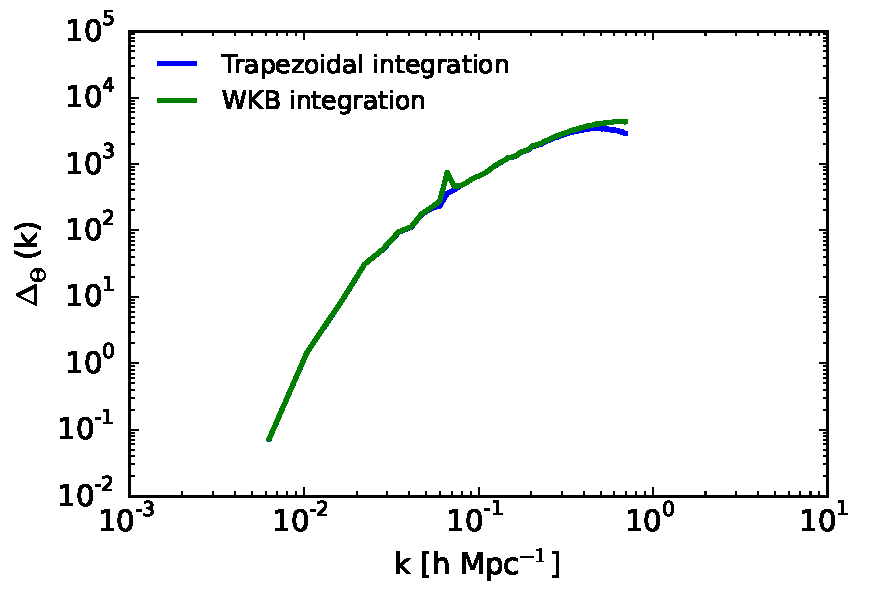
\includegraphics[width=0.495\textwidth]{Figures/wkb_v_0-eps-converted-to.pdf}}
  \subfloat[Error in WKB integration\label{fig:wkb_v_0_error}]{
    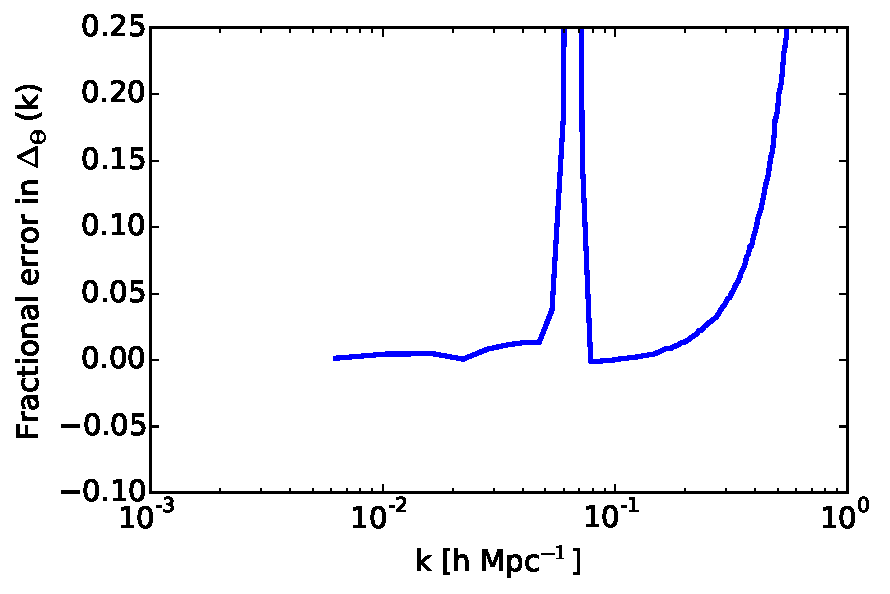
\includegraphics[width=0.495\textwidth]{Figures/wkb_v_0_error-eps-converted-to.pdf}}
  \caption{A comparison of the trapezoidal and WKB integration
    methods, specifically for the velocity divergence power of cold
    dark matter.  In figure \ref{fig:wkb_v_0}, the integration results
  are compared, while in figure \ref{fig:wkb_v_0_error} the fractional
error of the WKB method compared to the trapezoidal method is shown.}\label{fig:wkb_v}
\end{figure*}


In Figure \ref{fig:wkb_v}, we compare the results of the
trapezoidal and WKB integration method for the
reconstruction of the CDM velocity divergence power, a
case when the integrand is slowly varying and WKB integration is not
required.  Figure \ref{fig:wkb_v} shows that while this WKB integration
appears to be overly sensitive to some variations in the integrand, 
causing the spike at $k=0.07$ h Mpc$^{-1}$, overall the
method reproduces the integral with less than 25\% error up until
$k=0.5$ h Mpc$^{-1}$.  This isn't great, but things get worse when we try using this method to integration the density power spectrum. 

In Figure \ref{fig:wkb_den}, we compare the results of the trapezoidal and WKB integration method for the reconstruction of the CDM density power at z=0.  As you can see, the WKB integration method overestimates the integral by 30\% for $k>0.1$ h Mpc$^{-1}$.  Decreasing $d\tau''$ in Equation \eqref{eqn:wkb2} does not improve the results.

\begin{figure*}[h!]
  \centering
  \subfloat[Trapezoidal and WKB integrations\label{fig:wkb_den_0}]{
    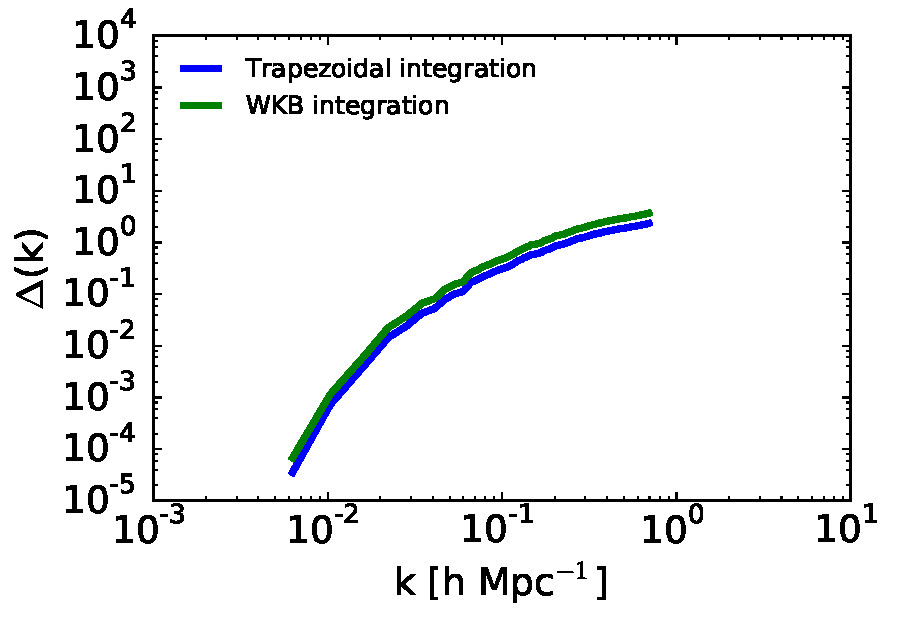
\includegraphics[width=0.495\textwidth]{Figures/wkb_0.pdf}}
  \subfloat[Error in WKB integration\label{fig:wkb_den_0_error}]{
    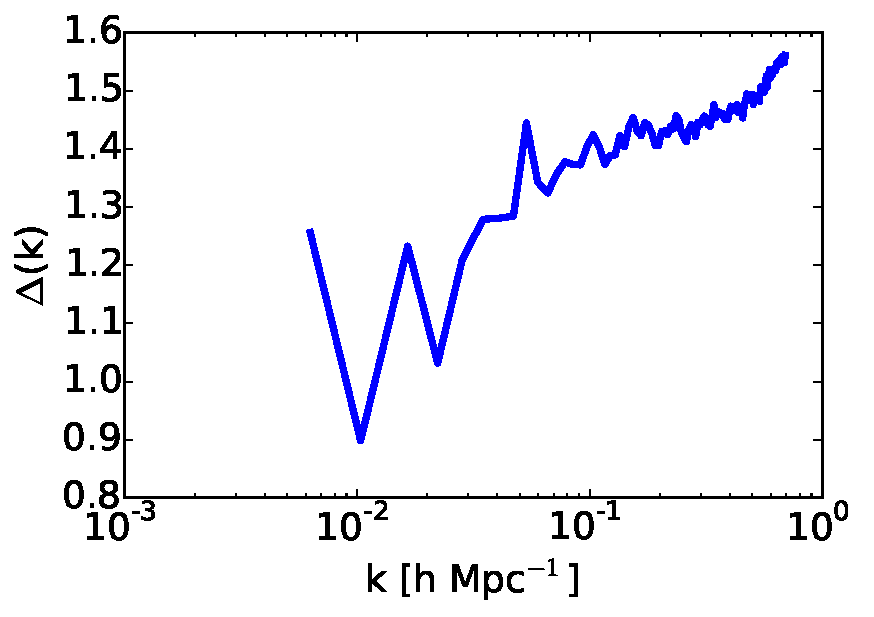
\includegraphics[width=0.495\textwidth]{Figures/wkb_0_error.pdf}}
  \caption{A comparison of the trapezoidal and WKB integration
    methods, specifically for the velocity divergence power of cold
    dark matter.  In figure \ref{fig:wkb_den_0}, the integration results
  are compared, while in figure \ref{fig:wkb_den_0_error} the fractional
error of the WKB method compared to the trapezoidal method is shown.}\label{fig:wkb_den}
\end{figure*}

\section{Variable interpolation scheme}
Next step is to try a variable interpolation scheme.  We have a varying function that we
are integrating over that contains $\sin ( k c_s (\tau - \tau') )$,
where we are integrating over $\tau$ from $\tau(z_0)$ to $\tau'$.  We
can calculate the number of oscillations that are in this function
from $\tau(z_0)$ to $\tau(z=0)$ or today.  This is given by:
\begin{equation}
  \mathrm{\#\;of\;oscillations} = \frac{ k c_s}{2 \pi}
  (\tau(z=0)-\tau(z_0))
\end{equation}
Say we want N sample points per oscillation, where N should be about
8-10.  Then we need a total number of points:
\begin{equation}
  \mathrm{ \#\;of\;sample\;points} = N \frac{ k c_s } {2 \pi}
  (\tau(z=0)-\tau(z_0)) 
\end{equation}
This is equivalent to performing the interpolation in $\tau$ space
instead of $t$ space.

For the density power, this is working well, as you can see in figure
\ref{fig:varinterp_den}.

\begin{figure*}
  \centering
  \caption{Results of using variable interpolation when calculating
    the neutrino density power.}\label{fig:varinterp_den}
  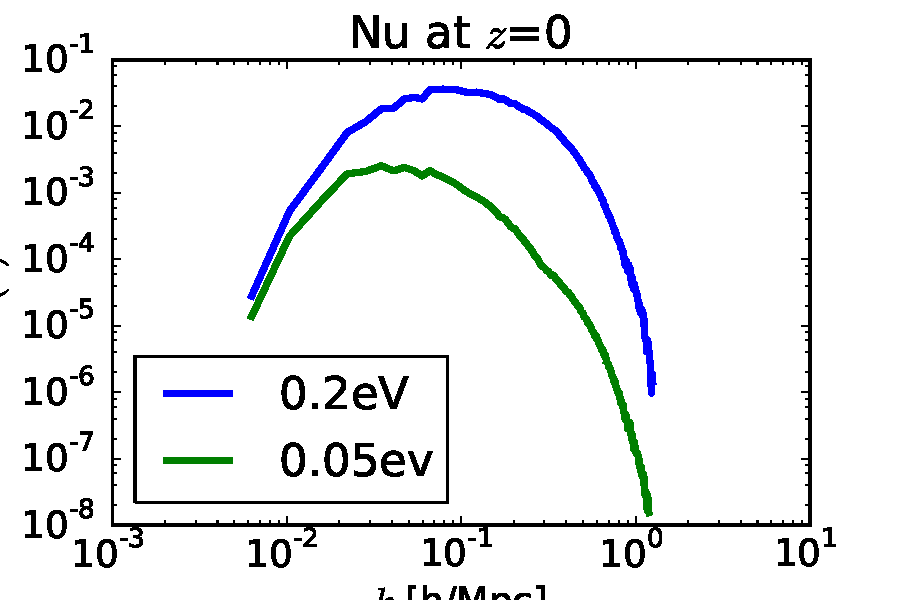
\includegraphics[width=0.6\textwidth]{Figures/density_nu_variable_interpolation.pdf}
\end{figure*}

\end{document}